\documentclass[12pt,oneside,letterpaper]{article}
\usepackage{float}
\usepackage{graphicx}
\usepackage[hidelinks]{hyperref}

% More powerful tables, incl. multi-page tables
\usepackage{longtable}
\usepackage{tabu}
% Ensure tabu tables can breathe
\global\tabulinesep=5pt

% Customization for enumerations
\usepackage{enumitem}

% Provide better unjustified text
\usepackage{ragged2e}

% Define single-spaced list
\newlist{compactenum}{enumerate}{2}
\setlist[compactenum]{label=\arabic*.,nosep}

% Define environment for single-spaced lists in tables
\newenvironment{packed_enumerate}{
\begin{minipage}[t]{\linewidth}\begin{compactenum}[after=\strut]}
{\end{compactenum}\end{minipage}}

% Expand the text area
\usepackage[textwidth=6.25in]{geometry}

\usepackage{titlesec}
\titleformat*{\paragraph}{\itshape}

% Set style on main pages
\pagestyle{headings}

\title{\bfseries PolitiMap: \\
Software Requirements Specification\\
version 4.0}

\author {\emph{CPE 307 Group 5}\\
\emph{California Polytechnic State University}\\
\emph{San Luis Obispo, CA USA}}

\date{October 13, 2016}

\begin{document}
\thispagestyle{empty}\maketitle
\newpage

\tableofcontents
\newpage

\section*{Credits}
\addcontentsline{toc}{section}{Credits}
\begin{tabu}{|X[.75]|l|X|l|}
\hline
\textbf{Name} & \textbf{Date} & \textbf{Role} & \textbf{Version} \\
\hline
Alanna Buss, Andrea Savage, Kevin Pham, Frank Poole, Michael Lenz, and Dat Tran & October 5, 2015 & Authors of template document & 1.0 \\
\hline
Yash Mehra & October 6, 2016 & Document Owner and Author & 1.1 \\
\hline
Andrew Gilbert & October 6, 2016 & Author & 1.1 \\
\hline
Jason Yoon & October 6, 2016 & Author & 1.1 \\
\hline
Devon Grove & October 6, 2016 & Author & 1.1 \\
\hline
Matt Goodrich & October 6, 2016 & Author & 1.1 \\
\hline
\end{tabu}

\section*{Revision History}
\addcontentsline{toc}{section}{Revision History}
\begin{tabu}{|X[L.5]|l|X|l|}
\hline
\textbf{Name}&\textbf{Date}&\textbf{Reason for Changes}&\textbf{Version} \\
\hline
Alanna Buss & October 13, 2016 & Initial format for requirements document & 1.0 \\
\hline
Yash Mehra & October 13, 2016 & Added introduction content and updated formating & 2.0 \\
\hline
Jason Yoon & October 13, 2016 & Added Use Cases & 2.1 \\
\hline
Jason Yoon and Matt Goodrich & October 14, 2016 & Added Flowchart & 2.2 \\
\hline
Yash Mehra & October 14, 2016 & Added System Requirements & 2.3 \\ 
\hline
Yash Mehra & October 14, 2016 & Added Non-Functional Requirements and External Interface Requirements & 2.4 \\
\hline
Yash Mehra & October 14, 2016 & Fixed Use Cases formatting & 3.0 \\
\hline
Jason Yoon & October 14, 2016 & Fixed External Interface Requirements and UI Requirements& 3.1 \\
\hline
Andrew Gilbert & October 14, 2016 & Added my use case and tweak formattng & 3.2 \\
\hline
Andrew Gilbert & October 14, 2016 & Proofreading and corrections. & 3.3\\
\hline
Name of person who does this & October 14, 2016 & Spelling, grammer and structure review. Final check for submission. & 4.0 \\
\hline
\end{tabu}

\newpage

\section{Introduction}
\subsection{Purpose}
This Software Requirements Specification describes the functional and nonfunctional software requirements for an application that brings local, regional and national political information to a user's mobile device.  This document is intended to be used by the members of the project team who will implement and verify the correct functionality of the system. This document will also be seen by our professor, Dr. Clark Turner.

\subsection{Intended Audience and Reading Suggestions}

\subsubsection{Software Development Engineers}
Developers will primarily reference the functional and nonfunctional requirements. These requirements correspond to the features to be implemented. For the purposes of implementation, it may also be helpful to reference use cases.

\paragraph{Suggested Reading Sequence:}
\begin{compactenum}
\item Overall Description
\item System Features
\item Use Cases
\item External Interface Requirements
\item Other Nonfunctional Requirements
\end{compactenum}

% I don't think we have any owners or customers right now --AG
\subsubsection{Software Product Owners and Customers}
Currently the developers are acting as customers, as they are members of the initial user class (i.e., young residents of San Luis Obispo).
%Customers will observe and confirm that the specified features and requirements meet business needs and that all user needs are brought to attention. Additionally, they will serve as the primary product owner as they will prioritize features during implementation.

%\paragraph{Suggested Reading Sequence:}
%\begin{compactenum}
%\item Overall Description
%\item System Features
%\item Use Cases
%\item External Interface Requirements
%\item Other Nonfunctional Requirements
%\end{compactenum}

\subsection{Project Scope}
Initially, the application will only provide a way of viewing current bills in the San Luis Obispo City Council.

Following a successful initial release, the next releases would be expected to add the ability to display current bills in the San Luis Obispo County Supervisors, followed by the California State Legislature and the US Congress. Push notifications would be added to notify people when a new bill is introduced. Further expansion to cover more geographical locations would be possible.

\subsection{References}
\begin{compactenum}
\item\href{https://docs.google.com/document/d/1hyrRutAoTPR2VO-z9vAM3607bGrHKqxODCZUUu3c8WM/edit}{Vision and Scope}
\end{compactenum}

\section{Overall Description}
\subsection{Product Perspective}
The application will provide local, regional and national political information based inputed and saved addresses the user provides. The information will be displayed in a clean, readable and simple format. User prefered locations will be saved, editited and deleted.

\subsection{Product Features}

\subsection{User Classes and Characteristics}
\begin{longtable}{|l|p{3.8in}|}
\hline
\textbf{User Class}&\textbf{Description}\\
\hline
Local Voters & Will be able to see policies that affect their everyday life as well as when said policies will be up for vote. Also can see different levels of policies.\\
\hline
Local activist groups & Make bills affecting their causes more widely known. Finding and supporting political figures that support their position.\\
\hline
Local government officials & Will recieve more calls from voters if the application succeeds. Not direct user of the application but directly affected by popularity of the application.\\
\hline
\end{longtable}

\subsection{Operating Environment}
This project will be run as an iPhone mobile application aimed at users across the United States. Since our initial target audience is limited to a domestic one, the geographic distribution won’t be such that servers at many unique locations will be necessary. Instead the application will request relevent information using Rest API calls to a backend that provides the information in simple JSON files. 

All information will be stored in JSON files since the data is static and is read only. Until the application scales to a much higher level and evolves into an interactive one, the need for setting up a secure database is unnecessary and is a waste of resources. For the scope of our project we have decided to set up the backend enviroment to meet the specifications and requirements in this way.

At this stage, we have not explored revenue streams for our business model besides advertising. At present, allowing user access for free somewhat reduces the risk incurred by a major service outage on our app since the degree of pressure involved when users pay for access to the application is significant. PolitiMap is not a tool we expect to be used more than once or twice a day by customers.

\subsection{Design and Implementation Constraints}
\begin{enumerate}
\item The application will be written in swift and thus initially only useable by users with a iPhone.
\item The backend with be written in ruby and will be accessebile to any front end with rest API calls.
\item The data is stored in JSON making front end to back end data transfer quick with no need for database access.
\end{enumerate}

\subsection{User Documentation}
TBD
\subsection{Assumptions and Dependencies}
\subsubsection{Assumptions}
\begin{enumerate}
\item More involvement with local politics is benecial
\item Voters lack information in order to be more involved with local politics
\item Voter involvement with local politics is limited
\end{enumerate}

\subsubsection{Dependencies}
\begin{enumerate}
\item Ability to get data on bills in a machine-parsable format (even if that is initially plaintext with custom code to parse it)
\end{enumerate}

\section{Use Cases}
\begin{longtable}{|r|p{3.8in}|}
\hline
Case ID & Description \\
\hline
1 & As a frequent traveler, I want to able to save multiple locations within the app so I can easily access the information on where I travel the most.\\
\hline
2 & As a Cal Poly student, I want to be able to view policy positions of local politicians so I can become encouraged to participate in local politics and make informed decisions in local elections.\\
\hline
3 & As a new voter, I want to be able to view previously-passed bills, so I can understand how politics have evolved and develop context for future bills. \\
\hline
4 & As an international student who is not familiar with US Politics, I want to be able to pinpoint bills that influence me, so I can be aware of my political position.\\
\hline
\end{longtable}


\begin{longtable}{|r|p{3.8in}|}
\hline
Use Case ID: & 1\\
  Use Case Name & Save Locations\\
  Created By & Yash Mehra\\
  Last Updated By & Yash Mehra\\
  Date Created & 2016-10-06\\
  Date Last Updated & 2016-10-06\\
  Actors & The PolitiMap App\\
  Description & Save multiple locations on the home page of the Application\\
  Preconditions &
  \begin{packed_enumerate}
  \item The location is currently supported by the app
  \item The app is open
  \item The app is on the home page
  \end{packed_enumerate} \\
  Postconditions &
  \begin{packed_enumerate}
  \item The app shows the saved location on the home page.
  \item The app should be able to access the location and show its Political information when tapped
  \end{packed_enumerate} \\
  Normal Flow &
  \begin{packed_enumerate}
  \item The user opens app
  \item The app loads locations saved by the user
  \item The user views saved locations
  \item (Alternative flow 1)
  \item The user searches a new locations
  \item The user chooses to save the location
  \end{packed_enumerate} \\
  Alternative Flows &
  Alternative flow 1
  \begin{packed_enumerate}
  \item Save location
  \end{packed_enumerate} \\
  Priority & High\\
  Special Requirements & \\
  Assumptions & All locations can be found\\
\hline
\end{longtable}

\begin{longtable}{|r|p{3.8in}|}
\hline
Use Case ID & 2\\
  Use Case Name & Display Policy Positions\\
  Created By & Devon Grove\\
  Last Updated By & Devon Grove\\
  Date Created & 2016-10-07\\
  Date Last Updated& 2016-10-07\\
  Actors & The PolitiMap App\\
  Description & View policy summary of given local politician on active issues\\
  Preconditions &
  \begin{packed_enumerate}
  \item The user's location is currently supported by the app
  \item The user has chosen the city council member to evaluate
  \item Push
  \item The user has selected "Policy Positions" from menu options
  \end{packed_enumerate} \\
  Postconditions &
  \begin{packed_enumerate}
  \item The app displays a summarized list of policy positions on active local legislation, and
  	lists a "position not available" message if position is indeterminate
  \end{packed_enumerate} \\
  Normal Flow &
  \begin{packed_enumerate}
  \item The user opens the app
  \item The user specifies their location, or a cached location is processed
  \item The user selects "Politicians" from the lower UI menu
  \item The user selects their chosen politician from the "Your Representatives" list
  \item The user navigates to "Policy Positions" using the UI menu
  \end{packed_enumerate} \\
  Priority & Medium\\
  Special Requirements & None\\
  Assumptions & Policy positions will be available publicly through government or council member's website\\
\hline
\end{longtable}

\begin{longtable}{|r|p{3.8in}|}
\hline
Use Case ID&3\\
Use Case Name&View Federal Bills\\
Created By&Matthew Goodrich\\
Last Updated By:&Matthew Goodrich\\
Date Created&October 6, 2016\\
Date Last Updated&October 6, 2016\\
Actors&The Application User; The Swift iOS Application; The Backend Server\\
Description&The application shall display a list of federal bills and further information about each upon selection.\\
Preconditions&
\begin{packed_enumerate}
\item The device is connected to the internet.
\item The backend is loaded with the organized data.
\item The device has the application downloaded, updated, and open to the home screen.
\item The backend server is running, whether it be an AWS component or EC2 instance.
\end{packed_enumerate}\\
Postconditions&
\begin{packed_enumerate}
\item A list of federal bills will be shown and likely scrolled-down, or the details of a specific bill will be showing.
\item A request will have been made to the AWS component or EC2 instance.
\item TBD - The federal bills may be cached in the user's device.
\end{packed_enumerate}\\
Normal Flow&
\begin{packed_enumerate}
\item The user chooses to view the list of bills relating to their local, state, and federal governments.
\item A GET request is made to the web server while the user sees a loading animation.
\item The user selects to filter the list of bills to show only federal bills.
\item The user scrolls through the bills and notices an interesting one.
\item The interesting bill is selected and the user reads related information, including a summary, associated representatives, and links to related external documentation.
\end{packed_enumerate}\\
Alternative Flow&
\begin{packed_enumerate}
\item The user selects a federal bills list instead of filtering a combined list.
\item The bills are loaded upon opening the application and only refreshed manually.
\item The bill information does not include associated representatives.
\item The bill shows dynamic data, such as votes and comments.
\end{packed_enumerate}\\
Exceptions&
\begin{packed_enumerate}
\item Unable to load the bills through the lack of an internet connection.
\end{packed_enumerate}\\
Includes&
\begin{packed_enumerate}
\item An external library to make the GET request.
\end{packed_enumerate}\\
Priority&High - One of the core functions of the application.\\
Frequency of Use:&Depends on the number of users and other variables.\\
Business Rules:&None\\
Special Requirements:&
\begin{packed_enumerate}
\item The application requests the data asynchronously.
\item The device is an iPhone 5 or newer.
\item Specific bill information is loaded with a GET request after a bill is selected.
\end{packed_enumerate}\\
Assumptions&
\begin{packed_enumerate}
\item Viewable federal bills exist in the backend.
\item Representatives have been linked to associated bills.
\item Documentation links have been added to associated bills.
\end{packed_enumerate}\\
Notes and Issues&None\\
\hline
\end{longtable}

\begin{longtable}{|r|p{3.8in}|}
\hline
Use Case ID & 4 \\
Use Case Name & View Bills that influences foreign students \\
Created By & Jason Yoon \\
Last Updated By & Jason Yoon \\
Date Created & October 6, 2016 \\
Date Last Updated & October 6, 2016 \\
Actors & 
\begin{packed_enumerate}
\item ios Application
\item The Back-End Server
\end{packed_enumerate}\\
Preconditions& 
\begin{packed_enumerate}
\item The device is connected to the internet and the app is downloaded.
\item The app is opened showing the main page.
\end{packed_enumerate}\\
Postconditions&
\begin{packed_enumerate}
\item One of the menu should direct the user to a new page.
\item The page will contain Bills that are related to foreign students.
\end{packed_enumerate}\\
Normal Flow &
\begin{packed_enumerate}
\item The user opens the app
\item The user navigates to the menu where it says "foreign students"
\item The user is able to scroll through the list of bills and save them in the bookmark
\end{packed_enumerate}\\
Alternative Flow & None \\
Special Requirements & None \\
Priority & Low \\
\hline
\end{longtable}

\begin{longtabu}{|r|p{3.8in}|}
\hline
  Use Case ID: & 1\\
  Use Case Name: & Display Agenda\\
  Created By: & Andrew Gilbert\\
  Last Updated By: & Andrew Gilbert\\
  Date Created: & 2016-10-06\\
  Date Last Updated: & 2016-10-06\\
  Actors: & The PolitiMap App\\
  Description: & Display the agenda for the next City Council meeting\\
  Preconditions: &
  \begin{packed_enumerate}
  \item The user has chosen a location which has a city council
  \item The location is currently supported by the app
  \item The app is open
  \item The user has chosen ``City Council Meeting'' from the list of events.
  \end{packed_enumerate} \\
  Postconditions: &
  \begin{packed_enumerate}
  \item The app shows the agenda for the next City Council meeting for
    the selected location.
  \end{packed_enumerate} \\
  Normal Flow: &
  \begin{packed_enumerate}
  \item The user opens app
  \item The app requests data from server
  \item (Alternative flow 1)
  \item The app displays a list of upcoming events
  \item The user chooses the City Council item
  \end{packed_enumerate} \\
  Alternative Flows: &
  Alternative flow 1
  
  \begin{packed_enumerate}
  \item Read data from cache
  \end{packed_enumerate} \\
  Priority: & High\\
  Special Requirements: & None\\
  Assumptions: & Council meeting agendas will be available for all
  supported locations\\
  Notes and Issues: & None\\
  \hline
\end{longtabu}
\section{Flowchart}
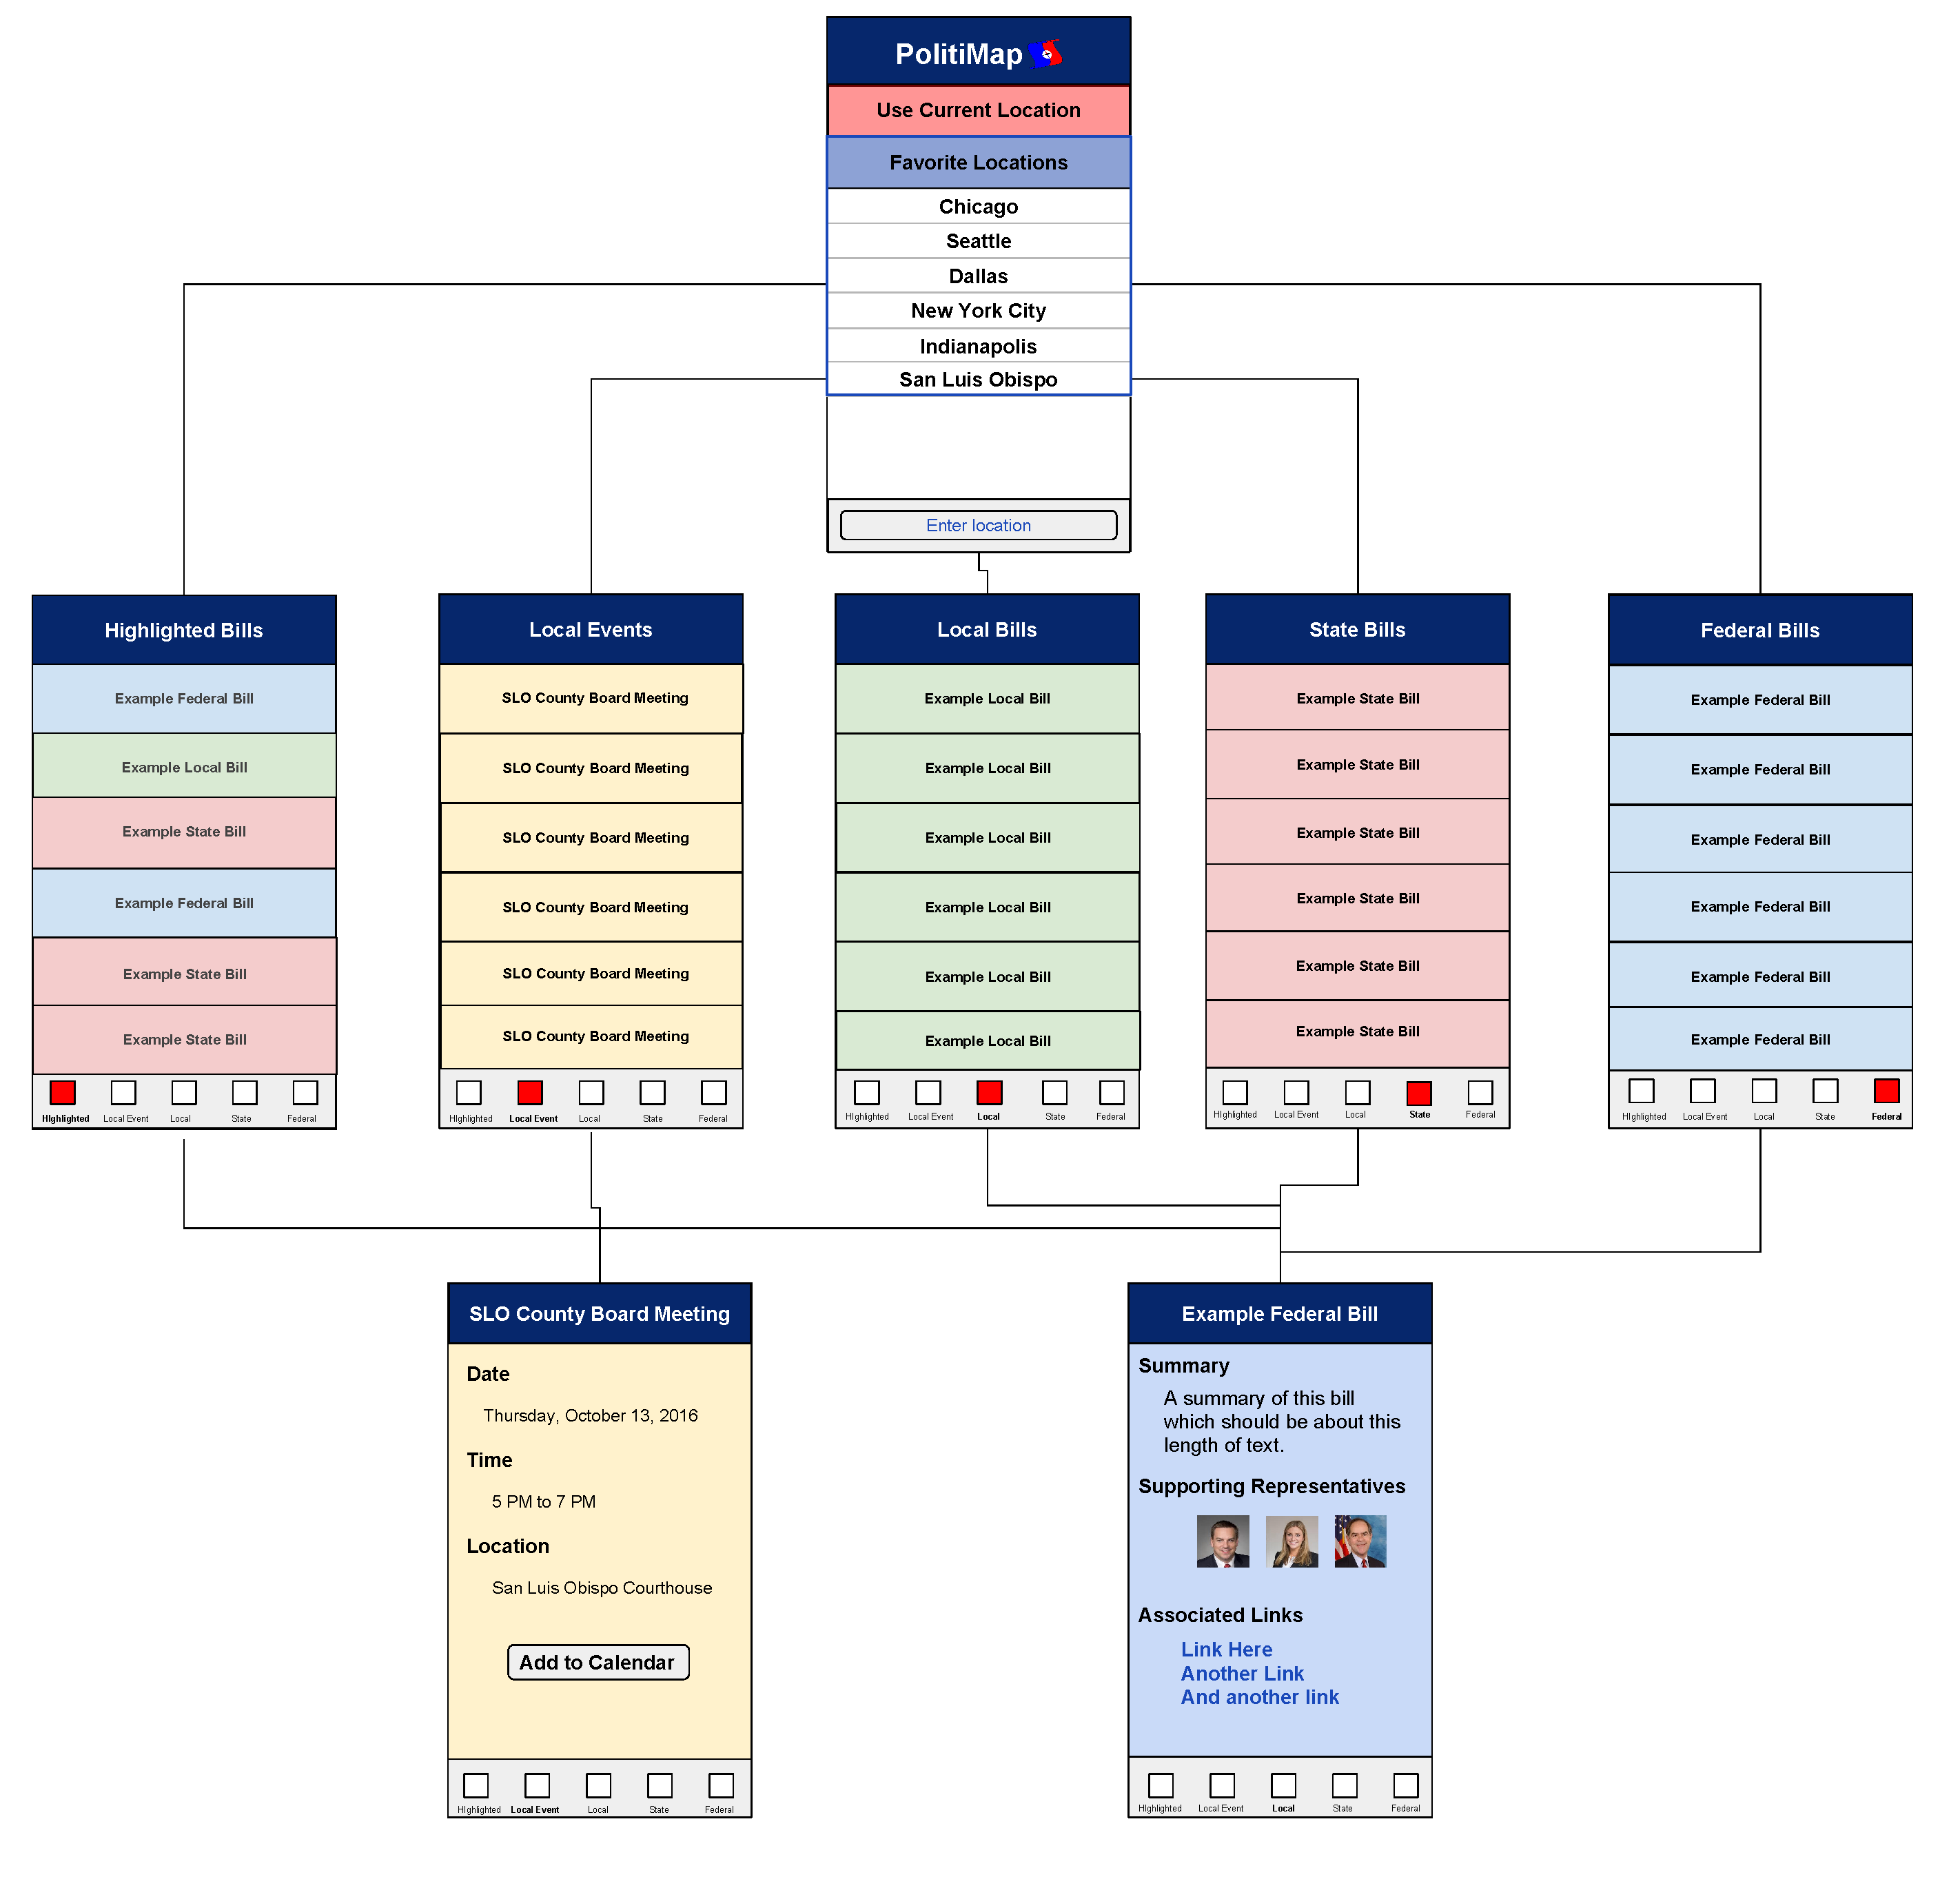
\includegraphics[width=\textwidth]{flowchart.pdf}

\section{System Features}

\subsection{Data Transmission}
\subsubsection{Description and Priority}
All data read by the application must be in the same format no matter the location. Data format must be standard at each locational level, local, regional or national. Data must be available to the system everytime a call is made.
\subsubsection{Stimulus/Response Sequences}
\begin{longtable}{|r|p{3.8in}|}
\hline
Stimulus & Once a location has been provided and the user has accesesed it the application will make a rest API call through the back end framework.\\
\hline
Response & The system will provide the correct data in the correct JSON format with a response to the Rest API call.\\
\hline
\end{longtable}
\subsubsection{Functional Requirements}
\begin{longtable}{|r|p{3.8in}|}
\hline
FR Requirement & Description \\
\hline
FR-1 & The system shall load data in the JSON format specied in an appendix. \\
\hline
FR-2 & The system shall fetch the data using AJAX or other method of web request. \\
\hline
FR-3 & The system shall only load JSON data for the locations
selected by the user. \\
\hline
FR-4 &The system shall data on politicians must be veriable and
completely accurate.\\
\hline
\end{longtable}

\subsection{Data editing}
\subsubsection{Description and Priority}
The user information is under the users full controll. The user should be able to add, edit and delete any user information. This is a big feature as in building an application for transparency. Users should feel in control. Users will not be able to edit requested data from saved locations, only the locations addresses themselves.
\subsubsection{Stimulus/Response Sequences}
\begin{longtable}{|r|p{3.8in}|}
\hline
Stimulus & User choses to edit address. \\
\hline
Response & Option to change address or delete it completely from the application. \\
\hline
\end{longtable}
\subsubsection{Functional Requirements}
\begin{longtable}{|r|p{3.8in}|}
\hline
FR Requirement & Description \\
\hline
FR-5 & The system should allow user locations to readable and writeable only locally. \\
\hline
\end{longtable}

\subsection{Data Logging}
\subsubsection{Description and Priority}
The system will store locally on the application the saved and preffered locations in the correct JSON format. They information stored will only be that off the address of the location. The information stored can be manipulated by the user.
\subsubsection{Stimulus/Response Sequences}
\begin{longtable}{|r|p{3.8in}|}
\hline
Stimulus & The application is on the home page and the user searches for a new address. \\
\hline
Response & The application verifies location and stores the new information. \\
\hline
\end{longtable}
\subsubsection{Functional Requirements}
\begin{longtable}{|r|p{3.8in}|}
\hline
FR Requirement & Description \\
\hline
FR-6 & The system should have a place for stored user locations. \\
FR-7 & The system should be able to read and write new data to the file according to the user preference. \\
\hline
\end{longtable}

\section{External Interface Requirements}

\subsection{User Interfaces}
For additional information about user interfaces, refer to the flowchart explained above.
\begin{longtable}{|r|p{3.8in}|}
\hline
UI Requirement & Description \\
\hline
UI-1 & The hompage will display a list of favorite locations and the search bar. It will also dispaly a menu to search based on the current location. \\
\hline
UI-2 & Highlighted Bills page will display a list of highlited Bills in Local, Federal, and State. In the bottom of the page, it will have tabs that link to other pages. It will also display the current page. \\
\hline
UI-3 & Local Events page will display a list of local events. In the bottom of the page, it will display tabs that link to other pages. It will also display what the current page is. \\
\hline
UI-4 & Local Bills page will display a list of local Bills. In the bottom of the page, it will display tabs that link to other pages. It will also display what the current page is.\\
\hline
UI-5 & State Bills page will display a list of State Bills. In the bottom of the page, it will display tabs that link to other pages. It will also display what the current page is.\\
\hline
UI-6 & Federal Bills page will display a list of Federal Bills. In the bottom of the page, it will display tabs that link to other pages. It will also display what the current page is.\\
\hline
UI-7 & Description page will display the details of selected item. It will also display tabs that link to other pages. \\
\hline
\end{longtable}

\subsection{Hardware Interfaces}
\begin{longtable}{|r|p{3.8in}|}
\hline
HI Requirement & Description \\
\hline
HI-1 & Mobile application is only for Iphones so user OS must be IOS and have access to Apple App Store. \\
\hline
\end{longtable}

\subsection{Software Interfaces}
\begin{longtable}{|r|p{3.8in}|}
\hline
SI Requirement & Description \\
\hline
SI-1 & The system shall update through the Apple App Store as new versions role out.\\
\hline
\end{longtable}

\section{Other Nonfunctional Requirements}

\subsection{Performance Requirements}
\begin{longtable} {|r|p{3.8in}|}
\hline
PR-1 & The system shall load the pages in under 2 seconds. \\
\hline
PR-2 & The system shall have zero memory leaks. \\
\hline
PR-3 & All bills will be updated within 1 day of recieving new information. \\
\hline
PR-4 & Memory should be availaible to store any new information \\
\hline
\end{longtable}

\subsection{Security Requirements}
\begin{longtable}{|r|p{3.8in}|}
\hline
CR-1 & User location information shall be secure. \\
\hline
\end{longtable}

\subsection{Software Quality Attributes}
\begin{longtable} {|r|p{3.8in}|}
\hline
SQ-1 & The system tests shall be repeatable and scalable. \\
\hline
\end{longtable}
\end{document}